\documentclass{ximera}
\author{Jenny Sheldon \and Bart Snapp}

\begin{document}
\begin{exercise}
  Here is a right triangle, note that it is \textbf{not} drawn to
  scale:
  \begin{image}
  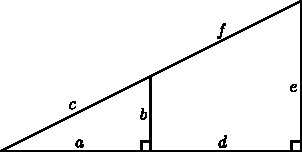
\includegraphics{origamiSimQ.pdf}
  \end{image}
  Solve for all unknowns in each of the following cases.
  \begin{enumerate}
  \item $a = 3$, $b = \answer{1}$, $c = \answer{\sqrt{10}}$, $d = 12$, $e = 5$, $f = \answer{4 \sqrt{10}}$
  \item $a = \answer{2.4}$, $b = 3$, $c = \answer{\sqrt{2.4^2+9}}$, $d =8$, $e = 13$, $f = \answer{\sqrt{169+10.4^2}-\sqrt{2.4^2+9}}$
  \item $a = 7$, $b = 4$, $c = \answer{\sqrt{65}}$, $d =\answer{77/4-7}$, $e = 11$, $f = \answer{\sqrt{11^2+(77/4)^2}-\sqrt{65}}$
  \item $a = 5$, $b = 2$, $c = \answer{\sqrt{29}}$, $d =6$, $e = \answer{22/5}$, $f = \answer{\sqrt{(22/5)^2+11^2}-\sqrt{29}}$
  \end{enumerate}
\end{exercise}
\end{document}
